\rightline{（文責:かりね）}
\section{ニート向け時間の潰し方Tier}
はじめまして、かりねと申します。今年の入寮パンフにはだめだめな記事が少ないと聞きました。熊野寮はかように肩肘張った雰囲気に一元化される場所ではありません。時間を持て余すニート歴4年目のこのわたくしに、だめだめな記事を担当させてくださいな。

しかし、締め切りはいま現在(午前3時)から1日もないらしい。そもそも最初の締め切りは2週間くらい前らしい。締め切りとゴムは加えた力に応じて十分に伸びますが、どちらにも限度があって、果てには壊れてしまうのです。いくらだめだめでも書かねばなりません。完全に昼夜が逆転しているので、次に起きた時に締め切りが過ぎていても文句は言えませんから、寝るまでに書き上げる決意を固めました。

幸いにも書きたいことは決まっていたので、タイトルから出来上がりました。「ニート向け時間の潰し方Tier」です。本当にだめそう。それでいてなぜかn575なのも面白い。去年退寮した先輩に「一生ダラダラし続けられるのもそれはそれで才能だと思うけどな」とのお言葉をいただく程には、時間の潰し方に心得があります。昨今の若者は生き急いでいます。関東の都会に生まれ育ちましたので、近傍の生の疾走感には驚くばかりでした。京都は時の流れがゆるやかで、それに浸って自分の心地よい拍子で鼓を打ってまいりました。二留しました、むべなるかな。ニート(NEET)がNot in Education, Employment, Trainingの略語なのは衆知と存じますが、大学にまるで行っていない以上は「Not in Education」の末席に加えていただきたい。末席という割には調子に乗って、タイトルの一単語目に抜擢しています。それでは以下、本題です。

% Tier表の準備 (tier_setup.texの内容)
\subsection{【問題のTier】}
公式ロゴといらすとやで食材を手に入れ、Tier表メーカー(\url{https://tier-list-maker-two.vercel.app/})様のお力添えのもと調理いたしました。左右差はあまり考えていません。いらすとやから画像を保存する過程で「neru\_man」とか「oshaberi\_man」とか愉快なファイル名が増えて、大変気分が良くなりました。嬉しい内容ではないけれど、「utsu\_man 」も面白い。構成要素ごとに軽く触れて仕舞を目指します。

\begin{figure}[h]
  \centering
  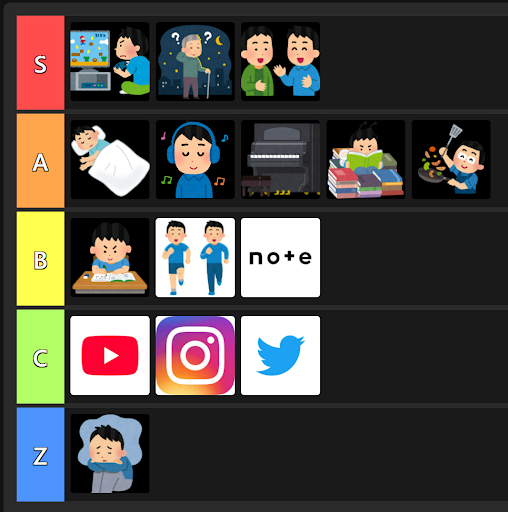
\includegraphics[width=0.9\linewidth]{2026shinki/neet_kill_time/images/Tier.png}
  \caption{ニート向け時間の潰し方Tier表}
\end{figure}

% S Tier (s_tier.texの内容)
\subsection{S Tier}
順にゲーム、深夜徘徊、雑談です。

\subsection*{ゲーム}
やはりニートといえばゲームです、とりわけオンラインゲーム。わたくしも多分に漏れることはなく、スマブラ、ポケモン、スプラトゥーン、雀魂etc.さまざまなタイトルに打ち込みました。最近は Shadowverse: Worlds Beyondを始めました。

% Shadowverseのランキング画像
\begin{figure}[h]
  \centering
  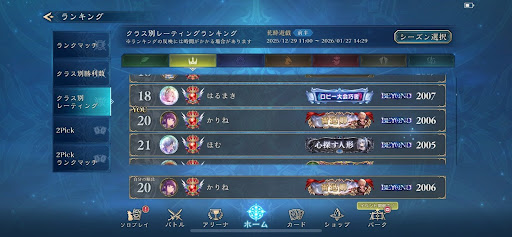
\includegraphics[width=0.8\linewidth]{2026shinki/neet_kill_time/images/shadowverse.jpg}
  \caption{Shadowverse: Worlds Beyond ランキング画面}
\end{figure}
最近始めたにしてはかなり強く、煌々と、あるいは妖々と輝くニートの証左です。対戦ゲームにおいては、なるべく先入観と偏見を排して環境を把握し、「優勢では負け筋を、劣勢では勝ち筋を探す」という発想でプレイングを反省し、ニートの時間を投資すると間違いなく勝てます。

\subsection*{深夜徘徊}
深夜徘徊は長らく続いている趣味で、京都の街とは素晴らしい相性です。ニートの持て余した余白と崩壊した生活習慣に対し、深夜に長距離を歩くという営みはかっちりはまり込んでいて、基質特異性のようです。去年の入寮パンフでは「深夜徘徊のすゝめ」というタイトルで寄稿いたしましたので、入寮後に折があればご一読くださいな。夜は落ち着きます、大好き。

\begin{figure}[h]
  \centering
  \begin{subfigure}{0.32\linewidth}
    \centering
    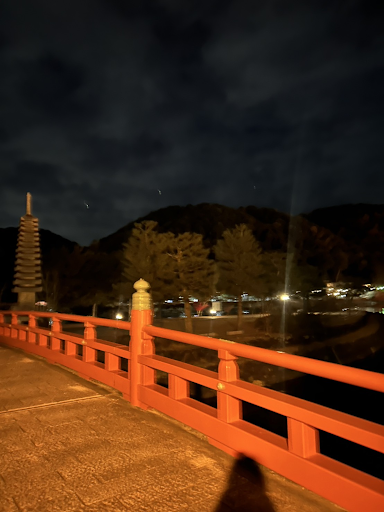
\includegraphics[width=\linewidth]{2026shinki/neet_kill_time/images/bridge.png}
    \caption{橋}
  \end{subfigure}
  \begin{subfigure}{0.32\linewidth}
    \centering
    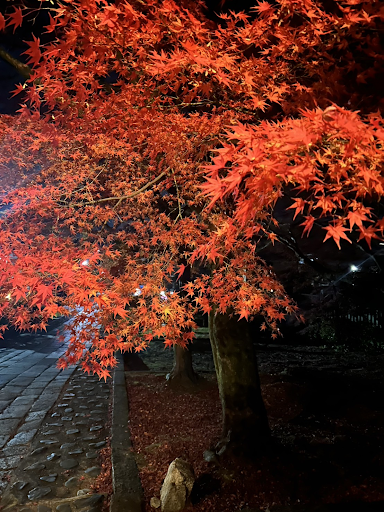
\includegraphics[width=\linewidth]{2026shinki/neet_kill_time/images/momiji.png}
    \caption{紅葉}
  \end{subfigure}
  \begin{subfigure}{0.32\linewidth}
    \centering
    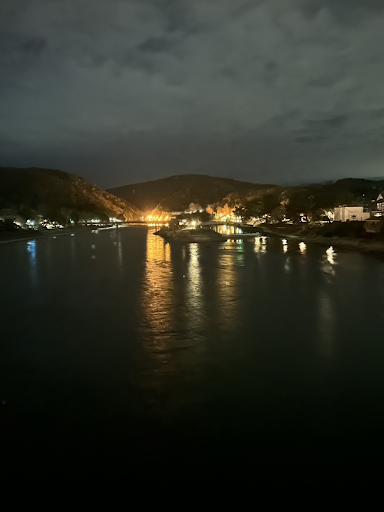
\includegraphics[width=\linewidth]{2026shinki/neet_kill_time/images/lake.png}
    \caption{湖}
  \end{subfigure}
  \caption{深夜徘徊中の風景}
\end{figure}

\subsection*{雑談}
雑談も特筆すべき時間つぶしです。友人とくだらない話で夜を明かすことは、4年経ったいまでも至福です。何も考えないで破綻したラリーを行う、通称「ランダム発話」が好みです。キャッチボールしているわけではなくて、各々一列に並んで壁打ちしているだけというシュールさが素晴らしい。

「コンビニ行かん?」への返答が「俺には感情がない」なとき、対話可能性の限界を垣間見ます。ちなみに彼はコンビニから帰るとスプラトゥーンを始め、「愛」と「恋」と「殺すぞ」を覚えました。

% A Tier (a_tier.texの内容)
\subsection{A Tier}
順に睡眠、音楽、楽器、読書、料理です。いずれもS Tierに劣らないポテンシャルを備えますが、熊野寮における全ニートに勧められるかどうかという観点から差を付けました。

\subsection*{睡眠}
ニートは眠っているばかりと口にする者は、非ニートの可能性が高いです。ニートは家から動かずに疲労が溜まらない日が多く、したがって睡眠時間は短い傾向にあります。正しくは強い主張として「横になっているばかり」、弱い主張として「家にいるばかり」なので、ニートに擬態する場合は参考にしてくだされば。それはそうとして、睡眠は重要です。ニートはその性質から精神や肉体を病むことが多いですが、睡眠は万病に効く薬ですので、意識的にその時間を確保すべきです。実は薬学部に所属しております、同志はお見知りおきくださいな。

\subsection*{音楽、楽器、読書}
音楽はひとを救う、言語を越えてゆけ。楽器や読書はニートと実に相性がよろしい。ニートにはいずれまったくやることのない虚無の時間が訪れますが、万人の想起する暇潰したるスマホやゲームの類は、少なくともその時点においてやり飽きています。これを楽器の練習や読書に変換することができれば、短期間で非凡な(非”非ニート”な)上達や陶冶を見ることとなります。

\subsection*{料理}
料理、わたくしにおいてはお菓子作りも、ニート性を十全に活かした営みです。時間がかかるという理由で敬遠されがちな品目は、ニートには垂涎の的に変貌します。否、美味しい料理ははなから垂涎ですね。甘美なるお菓子作りにぜひとも励みましょう。スコーンがね、また美味しいんだ。新歓で作るかもしれません。

\begin{figure}[h]
  \centering
  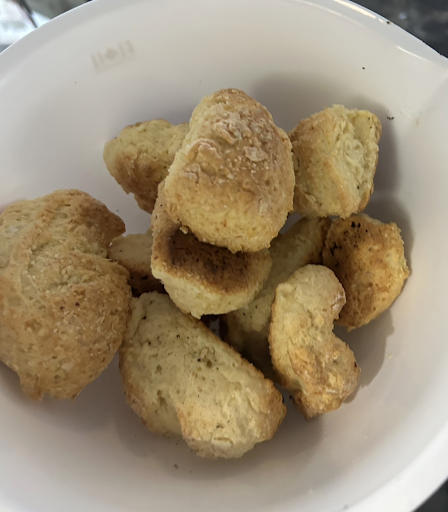
\includegraphics[width=0.25\linewidth]{2026shinki/neet_kill_time/images/cooking.png}
  \caption{料理・お菓子作りの様子}
\end{figure}